\section{Go's \unsafe{}~package}
\label{sec:background}

In this section, we give a brief introduction to \unsafe{} in Go and then present potential problematic code patterns including exploit information that we identified.

\subsection{Introducing \unsafe{}}
\label{sec:back:intro}

The Go programming language, like other memory-safe languages, provides an \unsafe{}~package\footnote{\url{https://golang.org/pkg/unsafe}}, which offers 
(a) the functions \textit{Sizeof}, \textit{Alignof}, and \textit{Offsetof} that are evaluated at compile time and provide access into memory alignment details of Go data types that are otherwise inaccessible, %unnecessary to know, and thus, inaccessible.
and (b) a pointer type, \textit{unsafe.Pointer} that allows developers to circumvent restrictions of regular pointer types.

One can cast any pointer to/from \textit{unsafe.Pointer}, thus enabling casts between completely arbitrary types, as illustrated in  
%
%In the remainders of this section, we discuss two example use cases of the \unsafe{} package in practice. 
Listing~\ref{lst:unsafe-ex-in-place-cast}.
%shows the usage of the \unsafe{} package to cast between arbitrary types.
In this example, \textit{in.Items} is assigned to a new type (\textit{out.Items}) in line 3 without reallocation for efficiency reasons. %\footnote{This code was taken from the Kubernetes \textit{k8s.io/apiserver} module with minor adjustments.} 
Furthermore, casts between \textit{unsafe.Pointer} and \textit{uintptr} are also enabled, mainly for pointer arithmetic.
A \textit{uintptr} is an integer type with a length sufficient to store memory addresses. 
However, it is not a pointer type, hence, not treated as a reference.
%The first \textit{unsafe.Pointer} rule allows casts between completely arbitrary types, and the latter one allows the use of pointer arithmetic.
%The usage of the \unsafe{}~package removes the safety net provided by the Go type system and compiler, and brings developers down to the flexibility and danger of the pointers in C.
%
Listing~\ref{lst:unsafe-ex-escape-analysis} presents an example of casts involving \textit{uintptr}. 
%The code is taken from the \textit{modern-go/reflect2} module.
In Line 2, the \textit{unsafe.Pointer} is converted to \textit{uintptr}.
Thus, the memory address is stored within a non-reference type.
Hence, the back-conversion in Line 3 causes the \textit{unsafe.Pointer} to be hidden from the \textit{escape analysis (EA)} which Go's garbage collector uses 
%manages the memory allocations and tries to identify memory which can be freed up.
%For this task, it uses \textit{escape analysis (EA)} 
to determine whether a pointer is local to a function and can be stored in the corresponding stack frame, 
or whether it can \textit{escape} the function and needs to be stored on the heap \cite{wang2020}. 
Since \textit{uintptr} values are not pointer types, storing the address of a pointer in a variable of such a type and then converting it back causes the \textit{EA} to miss the chain of references to the underlying value in memory. 
Therefore, Go will assume a value does not escape when it actually does, and may place it on the stack.
Correctly used it can improve efficiency because deallocation is faster on the stack than on the heap~\cite{wang2020}.
However, used incorrectly it can cause security problems as shown later in Section~\ref{sec:appr:vulnerabilites}.

\begin{lstlisting}[language=Golang, label=lst:unsafe-ex-in-place-cast, caption=In-place cast using the \unsafe{} package
from the Kubernetes \textit{k8s.io/apiserver} module with minor changes.
,float, belowskip=-1.5em]
func autoConvert(in *PolicyList, out *audit.PolicyList) error {
	// [...]
	out.Items = *(*[]audit.Policy)(unsafe.Pointer(&in.Items))
	return nil
}
\end{lstlisting}

\begin{lstlisting}[language=Golang, label=lst:unsafe-ex-escape-analysis, caption=Hiding a value from escape analysis from the \textit{modern-go/reflect2} module.
, float, belowskip=-1.5em]
func NoEscape(p unsafe.Pointer) unsafe.Pointer {
	x := uintptr(p)
	return unsafe.Pointer(x ^ 0)
}
\end{lstlisting}


% \subsection{Go Dependency Management}

%Old way: packages, Go Path

%New way: modules, registries, \textit{go.mod} file.

%Package cache, versions, bad reproducibility, relatively high error rates for dependency resolution.

%% ---------------------------------------------------

\subsection{Usage and Security Problems}
\label{sec:appr:vulnerabilites}

In the following, we discuss potential threat models and exploit vectors against real-world \unsafe{} Go code.
We present a code pattern in Listing~\ref{lst:string-to-bytes} that is very common in popular open-source Go projects (cf. Section~\ref{sec:eval}).
It is used to convert a string to a byte slice without copying the data.
As in Go strings essentially are read-only byte slices, this is commonly done by projects to increase efficiency of serialization operations. % and is possible as in Go, strings are essentially read-only byte slices.
Internally, each slice is represented by a data structure that contains its current length, allocated capacity, and memory address of the actual underlying data array.
The \textit{reflect} header structures provide access to this internal representation.
In Listing~\ref{lst:string-to-bytes} this conversion is done in line 2, 3, and 8 respectively.
First, an \textit{unsafe.Pointer} is used to convert a string to a \textit{reflect.StringHeader} type.
Then, a \textit{reflect.SliceHeader} instance is created and its fields are filled by copying the respective values from the string header.
Finally, the slice header object is converted into a slice of type \textit{[]byte}.

\begin{lstlisting}[language=Golang, label=lst:string-to-bytes, caption=Conversion from string to bytes using \unsafe{}, float, belowskip=-1.5em]
func StringToBytes(s string) []byte {
	strHeader := (*reflect.StringHeader)(unsafe.Pointer(&s))
	bytesHeader := reflect.SliceHeader{
		Data: strHeader.Data,
		Cap:  strHeader.Len,
		Len:  strHeader.Len,
	}
	return *(*[]byte)(unsafe.Pointer(&bytesHeader))
}
\end{lstlisting}


\subsubsection*{Implicit Read-Only}

The conversion pattern shown in Listing~\ref{lst:string-to-bytes} is efficient as it directly casts between \textit{string} and \textit{[]byte} in-place. %, without the need to reallocate the slice.
Using \textit{bytes := ([]byte)(s)} for the conversion would make the compiler allocate new memory for the slice header as well as the underlying data array.
However, the direct cast creates an implicitly read-only byte slice that can cause problems, as described in the following.
The Go compiler will place strings into a constant data section of the resulting binary file.
Therefore, when the binary is loaded into memory, the \textit{Data} field of the string header may contain an address that is located on a read-only memory page.
Hence, strings in Go are immutable by design and mutating a string causes a compiler error. %, alerting developers early in the development process that there is a problem.
However, when casting a string to a \textit{[]byte} slice in-place, the resulting slice loses the explicit read-only property, and thus, the compiler will not complain about mutating this slice although the program will crash if done so.
%Using this pattern, therefore, creates a trade-off between performance and potentially hard-to-find bugs that can lead to crashes.
%Due to the indirection resulting from the conversion to a slice which gets then passed around, they can be very hard to debug.


\subsubsection*{Garbage Collector Race}

Go uses a concurrent mark-and-sweep \textit{garbage collector (GC)} to free unused memory~\cite{sibiryov2017}.
It is triggered either by a certain increase of heap memory usage or after a fixed time. %, and runs in multiple parallel threads (Goroutines).
The GC treats pointer types, \textit{unsafe.Pointer} values, and slice/string headers as references and will mark them as still in use. %, preventing them from being freed.
Importantly, string/slice headers that are created manually as well as \textit{uintptr} values are not treated as references.
The last point, although documented briefly in the \textit{unsafe} package, is a major pitfall.
Casting a \textit{uintptr} variable back to a pointer type creates a potentially dangling pointer because the memory at that address might have already been freed if the GC was triggered right before the conversion.

Although not directly obvious, Listing~\ref{lst:string-to-bytes} contains such a condition.
Because the \textit{reflect.SliceHeader} value is created as a composite literal instead of being derived from an actual slice value, its \textit{Data} field is not treated as a reference if the GC runs between lines 3 and 8. 
Thus, the underlying data array of the \textit{[]byte} slice produced by the conversion might have already been collected.
This creates a potential \textit{use-after-free} or buffer reuse condition that, even worse, is triggered non-deterministically when the GC runs at just the "right" time.
%If the buffer is reused after being freed and the slice resulting from the cast is pointing to it, it can provide access to completely unrelated data. % even in concurrent Goroutines. 
Therefore, this race condition can crash the program, create an information leak, or even potentially lead to code execution.
Figure~\ref{fig:gcrace-vuln} shows a visualization of the casting process that leads to the problems described here.
The original slice is being cast to a string via some intermediate representations.
The slice header is shown in green (at memory position 1), while the underlying data array (memory position 2) is shown in red.
When the resulting string header (shown in blue at memory position 3) is created, it only has a weak reference to the data, and when the GC runs before converting it to the final string value, the data is already freed.

\begin{figure}[!t]
    \vspace{2mm}
    \centering
    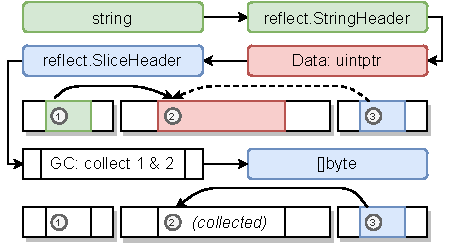
\includegraphics[width=0.4\textwidth]{gfx/figures/gcrace-vuln.pdf}
    %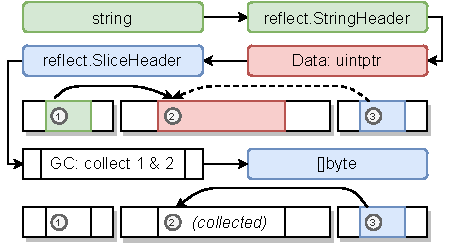
\includegraphics[width=0.48\textwidth]{gfx/figures/gcrace-vuln.pdf}
    \caption{GC race and escape analysis flaw}
    \label{fig:gcrace-vuln}
    \vspace{-8pt}
\end{figure}



\subsubsection*{Escape Analysis Flaw}

A third problem found in Listing~\ref{lst:string-to-bytes} is that the \textit{escape analysis (EA)} algorithm can not infer a connection between the string parameter \textit{s} and the resulting byte slice.
Although, they use the same underlying data array, the EA misses this due to the fact that the intermediate representation as a \textit{uintptr} is not treated as a reference type.
This can cause undefined behavior if the returned value from the casting function is used incorrectly.

Listing~\ref{lst:escape-analysis} shows a program that uses the conversion function presented earlier~(Listing~\ref{lst:string-to-bytes}).
In the \textit{main} function, \textit{GetBytes} is called~(Line 2), which creates a string and turns it into a byte slice using the conversion function.
Within the \textit{GetBytes} function, we create the string using a \textit{bufio} reader similarly to if it were user-provided input.
After the cast, \textit{GetBytes} prints the resulting bytes~(Line 10) and returns them to \textit{main}, which also prints the bytes~(Line~3).
Although, one might assume that both print statements result in the same string to be displayed, the second one in \textit{main} fails and prints invalid data.


% // expected (but failed) stdout is "abcdefgh
% // expected stdout is "abcdefgh"
\begin{lstlisting}[language=Golang, label=lst:escape-analysis, caption=Escape analysis flaw example, float, belowskip=-1.5em]
func main() {
	bytesResult := GetBytes()
	fmt.Printf("main: %s\n", bytesResult)
}

func GetBytes() []byte {
	reader := bufio.NewReader(strings.NewReader("abcdefgh"))
	s, _ := reader.ReadString('\n')
	out := StringToBytes(s)
	fmt.Printf("GetBytes: %s\n", out)
	return out
}
\end{lstlisting}

Because the string \textit{s} is allocated in \textit{GetBytes} the Go EA is triggered. %try to figure out if it escapes.
It concludes that \textit{s} is passed to \textit{StringToBytes} and the EA transitively looks into that function.
Here, it fails to connect \textit{s} to the returned byte slice as described previously.
Therefore, the EA concludes that \textit{s} does not escape in \textit{StringToBytes}.
As it is not used after the call in \textit{GetBytes}, the EA algorithm incorrectly assumes that it does not escape at all and places \textit{s} on the stack.
When \textit{GetBytes} prints the resulting slice, the data is still valid and the correct data is printed, but once the function returns to \textit{main}, its stack is destroyed.
Thus, \textit{bytesResult} (Line~2) is now a dangling pointer into the former stack of \textit{GetBytes} and, therefore, printing data from an invalid memory region.


%\subsubsection*{Correct In-Place Cast}
%
%To avoid the problems described in the previous sections, it is crucial to not create instances of \textit{reflect.SliceHeader} and \textit{reflect.StringHeader} from scratch, instead they must be derived from actual slices or strings.
%Although this is documented with the \textit{unsafe} package, there are many incorrect usages in the projects we analyzed.
%A correct version of the in-place cast is shown in Listing~\ref{lst:correct-slice-cast}.
%
%\begin{lstlisting}[language=Golang, label=lst:correct-slice-cast, caption=Correct in-place string to bytes cast]
%func StringToBytes(s string) (b []byte) {
%	strHeader := (*reflect.StringHeader)(unsafe.Pointer(&s))
%	bytesHeader := (*reflect.SliceHeader)(unsafe.Pointer(&b))
%	bytesHeader.Data = strHeader.Data
%	bytesHeader.Cap = strHeader.Len
 %   bytesHeader.Len = strHeader.Len
%	return
%}
%\end{lstlisting}
\begin{figure}[htp!]
    %\vspace{2mm}
    \centering
    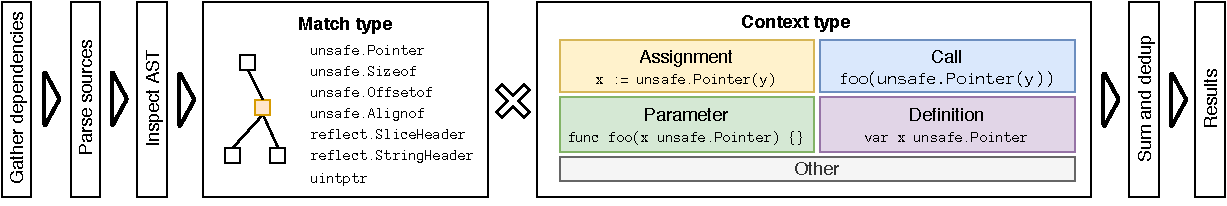
\includegraphics[width=\textwidth]{assets/figures/chapter4/go-geiger-architecture.pdf}
    \caption{Architecture of the \toolGeiger{} tool to detect unsafe usages}
    \label{fig:geiger-architecture}
    %\vspace{-10pt}
\end{figure}



\subsubsection*{Code Execution}

To show the severity of the issues identified above and that they are not just of theoretical nature, e.g., resulting in simple program crashes, we created a proof of concept for a code execution exploit using \textit{Return Oriented Programming (ROP)} on a vulnerable \unsafe{} usage. %vulnerability caused by a misuse of \unsafe{}.
The sample incorrectly casts an array on the stack into a slice without constricting it to the proper length.
This vulnerability causes a buffer overflow which we use to overwrite the stored return address on the stack, thus, changing the control flow of the program. 
Since Go programs are typically statically linked with a big runtime, there is a large number of ROP-gadgets available within the binary itself. 
We use gadgets to set register values and dispatch to system calls. 
Using the \textit{mprotect} syscall, we set both the writable and executable permission bits on a memory page that is mapped to the program, and store an exploit payload provided via standard input there using the \textit{read} syscall. 
Finally, we jump to this payload and execute it using a final ROP-gadget to open a shell.
An in-depth discussion of the exploit would go beyond the scope of this paper and exceed the space available to present our research.
Therefore, we made it available online\footnote{\url{https://github.com/jlauinger/go-unsafepointer-poc}\label{fn:poc}} together with five other proof-of-concepts. 

